\documentclass[11pt,a4paper]{article}

% ==============================================================================
% PACKAGES & PAGE GEOMETRY
% ==============================================================================
\usepackage[utf8]{inputenc}
\usepackage[T1]{fontenc}
%\usepackage{lmodern}
\usepackage[expansion=false]{microtype}
\usepackage[margin=1in]{geometry}
\usepackage{amsmath,amssymb,amsfonts,amsthm,mathtools}
\usepackage{bm}
\usepackage{booktabs}
\usepackage{multirow}
\usepackage{array}
\usepackage{algorithm}
\usepackage{algpseudocode}
\usepackage{xcolor}
\usepackage{tikz}
\usetikzlibrary{arrows.meta,positioning,shapes.geometric,calc,fit,backgrounds}
\usepackage[colorlinks=true,linkcolor=blue!70!black,citecolor=teal!70!black,urlcolor=blue!70!black]{hyperref}

% ==============================================================================
% THEOREM ENVIRONMENTS & MATHEMATICAL MACROS
% ==============================================================================
\newtheorem{theorem}{Theorem}[section]
\newtheorem{proposition}[theorem]{Proposition}
\newtheorem{lemma}[theorem]{Lemma}
\newtheorem{corollary}[theorem]{Corollary}
\theoremstyle{definition}
\newtheorem{definition}[theorem]{Definition}
\theoremstyle{remark}
\newtheorem{remark}[theorem]{Remark}

\newcommand{\R}{\mathbb{R}}
\newcommand{\C}{\mathbb{C}}
\newcommand{\Ha}{\mathbb{H}}
\newcommand{\Oc}{\mathbb{O}}
\newcommand{\Se}{\mathbb{S}}
\newcommand{\Ftwo}{\mathbb{F}_2}
\newcommand{\PG}{\mathrm{PG}}
\newcommand{\ImPart}{\mathrm{Im}}
\newcommand{\RePart}{\mathrm{Re}}
\newcommand{\Aut}{\mathrm{Aut}}
\newcommand{\rank}{\mathrm{rank}}
\newcommand{\Null}{\ker}
\newcommand{\Falt}{\mathcal{F}_{\mathrm{alt}}}
\newcommand{\Fzd}{\mathcal{F}_{\mathrm{ZD}}}
\newcommand{\PiMoreno}{\Pi_{\mathrm{Moreno}}}
\newcommand{\PiNull}{\Pi_{\ker L}}
\newcommand{\popcount}{\mathrm{popcount}}

% ==============================================================================
% TITLE & AUTHOR METADATA
% ==============================================================================
\title{\textbf{Sedenion Algebras and $\PG(3,2)$ Incidence Structures\\
for Non-Associative Geometric Deep Learning:\\
Algebraic Foundations, Machine-Checked Theorems, and Dual-Track Validation}}

\author{
  \textbf{Dionisio Chiuratto Agourakis}\thanks{Correspondence: \href{mailto:dionisio.ca@gmail.com}{\texttt{dionisio.ca@gmail.com}}.} \\[0.4em]
  \small \href{mailto:dionisio.ca@gmail.com}{\texttt{dionisio.ca@gmail.com}}
}

\date{October 2026}

\begin{document}

\maketitle

% ==============================================================================
% ABSTRACT
% ==============================================================================
\begin{abstract}
\noindent
Modern geometric deep learning architectures operate predominantly over associative division algebras---the reals ($\R$), complexes ($\C$), and quaternions ($\Ha$)---with limited extensions to the 8-dimensional alternative octonions ($\Oc$). Proceeding one step further along the Cayley--Dickson tower to the 16-dimensional sedenions ($\Se = \Oc \oplus \Oc e_8$) simultaneously breaks associativity, alternativity, and the division property, introducing a rich submanifold of non-trivial zero divisors. While historically treated as numerical pathologies, we argue that non-associativity and zero-divisor annihilation can provide a mathematically rigorous geometric inductive bias for both theoretical physics surrogates and neuro-symbolic normative reasoning. 

First, we establish a \textbf{Differentiable Sedenion Calculus}, proving the \textit{Universal Cayley--Dickson Adjoint Theorem} ($L(w)^\top = L(w^*)$ and $R(x)^\top = R(x^*)$), which enables exact backpropagation through $16\times$ parameter-compressed sedenion layers without materializing $16M \times 16N$ Jacobian matrices in High Bandwidth Memory (HBM). Second, we embed the 15 imaginary basis units of $\Se$ into the finite projective 3-space $\PG(3,2)$ and prove the \textbf{$8+7$ Fano Hyperplane Bifurcation Theorem}: the 15 Fano planes ($\PG(2,2)$) of $\Se$ partition into 8 norm-preserving alternative octonion workspaces ($\Falt \cong \Oc$, internally zero-divisor-free) and 7 quasi-octonion workspaces ($\Fzd \cong \tilde{\Oc}$), each of which contains complete annihilating pairs; the 21 mixed projective lines hosting the Moreno--Stiefel zero-divisor cone $V_2(\R^7)$ each lie in two $\Fzd$ workspaces and one $\Falt$ workspace. Furthermore, any two Fano workspaces intersect in a unique 3-node associative quaternion hinge $L_{12} \cong \Ha$, guaranteeing working-memory continuity during context switches. Third, we design hardware-sympathetic GPU/ONNX kernels utilizing 4-bit ALU XOR index swizzling ($i = k \oplus j$) and 256-bit register-packed IEEE-754 sign-bit flips. Fourth, we prove a constructive \textbf{4D Moreno Nullspace Projection Theorem} that maps overriding premises directly into $\ker L(u)$, eliminating probabilistic ``softmax bleed'' to floating-point round-off (mean $2.4 \times 10^{-16}$ in FP64, $1.4 \times 10^{-7}$ in FP32, measured over $1{,}024$ samples). All algebraic claims are verified by an accompanying test-suite, and their finite content (the Cayley--Dickson structure constants, the adjoint sign identities, the $\PG(3,2)$ bifurcation, explicit zero divisors, the $672/2520$ basis associator census, and the $\Falt/\Fzd$ cyclic BCJ stratum theorems) is machine-checked in Lean~4 without \texttt{sorry} or \texttt{native\_decide} (64 theorems), while the constructive nullspace theorem and its converse ($\operatorname{rank} L(u) = 12$) are proved over $\R$ in Lean~4/Mathlib. Finally, we empirically validate both Track A and Track B benchmarks: (1) on Track A 4-gluon Yang--Mills color-kinematics scattering (\texttt{bench/track\_a}), our $\PG(3,2)$-routed \texttt{Sed-PG32-Moreno} surrogate achieves a BCJ Jacobi violation residual of $\mathcal{R}_{\mathrm{BCJ}} = 1.8 \times 10^{-8}$ and a collinear pole relative error of $\mathcal{E}_{\mathrm{pole}} = 6.9 \times 10^{-3}$ at $|s_{ij}| < 10^{-4}$ (versus $\mathcal{R}_{\mathrm{BCJ}} = 0.58\text{--}0.76$ and $\mathcal{E}_{\mathrm{pole}} > 4 \times 10^3$ for Softmax, $\Ha^4$, $\Oc^2$, and $\mathcal{Cl}_{0,4}$ baselines); and (2) on Track B multi-hop normative contradiction pruning (\texttt{bench/gate3}, $\mathrm{aux}=0.0$), Sedenion Zero-Divisor Attention achieves \textbf{$100.0\%$ ID accuracy ($d \in \{0,1,2\}$), $100.0\%$ OOD depth generalization ($d=3, 4$), $0.0\%$ False-Compliance Rate (FCR), and $2.1 \times 10^{-10}$ attention leakage}, including in the parameter-halved ``No-FFN'' regime \cite{Ji2026CliffordNet} ($-47.4\%$ parameters).
\end{abstract}

\noindent\textbf{Keywords:} Cayley--Dickson Algebras, Sedenions, Zero Divisors, Finite Projective Geometry $\PG(3,2)$, Fano Plane, Exceptional Lie Group $G_2$, Geometric Deep Learning, Neuro-Symbolic Normative Reasoning.

\vspace{1em}
\hrule
\vspace{1.5em}

% ==============================================================================
% SECTION 1: INTRODUCTION
% ==============================================================================
\section{Introduction}
\label{sec:intro}

The expressive efficiency of a neural architecture is governed by the algebraic structure of its underlying representation space \cite{Bronstein2021}. Extending real-valued networks ($\R$) to complex ($\C$, 2D) \cite{Trabelsi2018} and quaternionic ($\Ha$, 4D) \cite{Parcollet2019} representations replaces unconstrained dense weight matrices with structured Hamilton products, yielding a $2\times$ and $4\times$ reduction in free parameters alongside improved inter-channel phase coupling. By Hurwitz's theorem, the normed division algebras over $\R$ terminate at the 8-dimensional octonions ($\Oc$) \cite{Baez2002,Schafer1966}, which forfeit associativity in favor of the weaker property of \textit{alternativity} ($x(xy) = (xx)y$ and $(yx)x = y(xx)$).

Applying the Cayley--Dickson doubling construction \cite{Cayley1845,Dickson1919} a fourth time produces the 16-dimensional \textbf{sedenions} ($\Se$). Unlike $\R, \C, \Ha$, and $\Oc$, the algebra $\Se$ is neither alternative nor a division algebra: it possesses non-trivial \textbf{zero divisors}---pairs of non-zero elements $u, v \in \Se \setminus \{0\}$ whose product vanishes identically ($u \cdot v = 0$) \cite{Moreno1998}. In classical numerical analysis, zero divisors and non-associativity are viewed as obstructions because they invalidate standard matrix inversion, norm multiplicativity ($\|u \cdot v\|_2 \neq \|u\|_2 \|v\|_2$), and order-independent chain rules.

In this paper, we invert this perspective. Building upon recent combinatorial characterizations of zero-divisor-free coordinate cells and projective bitmask operators in the Cayley--Dickson tower \cite{Agourakis2026a,Agourakis2026b}, we argue that the algebraic anomalies of $\Se$ address two bottlenecks in modern artificial intelligence and computational physics:
\begin{enumerate}
    \item \textbf{Probabilistic Attention Bleed in Normative and Symbolic Reasoning:} Standard Transformer attention mechanisms rely on strictly positive softmax distributions ($\alpha_{ij} > 0$). When auditing complex statutory or financial hierarchies (e.g., securities regulations where a specific safe-harbor or prohibition strictly invalidates a general rule), invalidated clauses retain non-zero attention weight that compounds across reasoning hops. By projecting mutually exclusive premises onto the \textit{Moreno zero-divisor manifold} in $\Se$, contradictory states can be made to annihilate exactly ($u \cdot v = 0$) at the tensor level, without post-hoc masking.
    \item \textbf{Order-Invariance vs.\ Context-Dependent Precedence:} Associative matrix multiplication satisfies $(AB)C = A(BC)$, rendering standard linear layers blind to the hierarchical parenthesization of triadic interactions unless aided by positional heuristics. In $\Se$, the associator $[u, v, w] = (u \cdot v) \cdot w - u \cdot (v \cdot w)$ is governed by the incidence geometry of the 15-point projective 3-space $\PG(3,2)$: collinear triads associate strictly ($[u, v, w] = 0$), whereas non-collinear triads have a generically non-zero associator (1{,}848 of the 2{,}520 ordered non-collinear basis triads; the remaining $672 = 7 \times 96$ associate because they are the adjacent-stratum $L_0 \sqcup Q_1$ triads of the 7 quasi-octonion Fano planes $\Fzd$).
\end{enumerate}

\subsection*{Summary of Contributions}
\begin{itemize}
    \item \textbf{Differentiable Sedenion Calculus \& Moreno Geometry (\S\ref{sec:wp1}):} We formulate left/right multiplication operators in $\Se$, parameterize non-associative parenthesization via a differentiable operator commutator gate $\mathcal{M}_\alpha$, and prove the \textit{Universal Cayley--Dickson Adjoint Theorem} (Theorem~\ref{thm:adjoint}), enabling $O(1)$-expansion backpropagation.
    \item \textbf{$\PG(3,2)$ Topological Routing \& The $8+7$ Fano Bifurcation (\S\ref{sec:wp2}):} We prove that the 15 Fano hyperplanes of $\PG(3,2)$ embedded in $\Se$ bifurcate into 8 alternative octonion workspaces ($\Falt \cong \Oc$) and 7 quasi-octonion zero-divisor workspaces ($\Fzd \cong \tilde{\Oc}$) connected by 3-node associative quaternion hinges (Theorems~\ref{thm:fano_bifurcation} and \ref{thm:hinge}).
    \item \textbf{Zero-Expansion Hardware Kernels (\S\ref{sec:wp3}):} We design and verify zero-expansion sedenion kernels that eliminate the $16\times$ weight-materialization bottleneck ($136.0\,\mathrm{MB} \to 8.0\,\mathrm{MB}$ for $4096 \times 4096$ layers), using 4-bit ALU XOR index swizzling and 256-bit register-packed IEEE-754 sign-bit operations for PyTorch, Triton, and ONNX Runtime.
    \item \textbf{Constructive 4D Nullspace Projector, BCJ/Half-Sphere Theorems \& Dual-Track Validation (\S\ref{sec:wp4}):} We derive a closed-form analytical operator $\PiNull(u)$ mapping any vector in a 4D orthogonal complement into $\ker L(u)$ (Theorem~\ref{thm:nullspace}), prove both the \textit{$\Fzd$ BCJ Numerator \& Collinear Pole Cancellation Theorem} (Theorem~\ref{thm:bcj_pole}) and the \textit{Orthogonal Half-Sphere Key Modulation Theorem} (Theorem~\ref{thm:half_sphere}), and empirically validate Track A (Yang--Mills BCJ scattering: $\mathcal{R}_{\mathrm{BCJ}} = 1.8 \times 10^{-8}$, $\mathcal{E}_{\mathrm{pole}} = 6.9 \times 10^{-3}$) and Track B (multi-hop contradiction pruning: $100.0\%$ ID/OOD accuracy, $0.0\%$ FCR, and $2.1 \times 10^{-10}$ leakage across standard and \texttt{No-FFN} \cite{Ji2026CliffordNet} backbones).
\end{itemize}

% ==============================================================================
% SECTION 2: DIFFERENTIABLE SEDENION CALCULUS (WP1)
% ==============================================================================
\section{Differentiable Sedenion Calculus and Zero-Divisor Geometry}
\label{sec:wp1}

\subsection{Cayley--Dickson Doubling and XOR Structure Constants}
Let $\Se$ denote the 16-dimensional real sedenion algebra spanned by the canonical orthonormal basis $E = \{e_0, e_1, \dots, e_{15}\}$, where $e_0 = 1$ is the multiplicative identity and $e_1, \dots, e_{15}$ are imaginary units satisfying $e_i^2 = -e_0$ and $e_i e_j = -e_j e_i$ for all distinct $i, j \in \{1, \dots, 15\}$. Under the Cayley--Dickson construction $\Se = \Oc \oplus \Oc e_8$, any sedenion $u \in \Se$ decomposes into an ordered pair of octonions $u = (a, b) = a + b e_8$ with $a, b \in \Oc$, multiplying via:
\begin{equation}
\label{eq:cd_doubling}
(a, b) \cdot (c, d) = \big(a c - d^* b, \;\; d a + b c^*\big),
\end{equation}
where $x^* = x_0 e_0 - \sum_{i=1}^{15} x_i e_i$ denotes the involutive conjugate and $\langle u, v \rangle = \RePart(u^* \cdot v) = \sum_{k=0}^{15} u_k v_k$ is the canonical Euclidean inner product on $\R^{16} \cong \Se$.

\begin{definition}[Bitwise XOR Multiplication Law and Operator Matrices]
\label{def:xor_mult}
Indexing the basis $E$ by 4-bit binary integers $i, j \in \{0, \dots, 15\} \cong \Ftwo^4$, the product of any two basis units is closed under bitwise exclusive-OR ($\oplus$):
\begin{equation}
\label{eq:basis_xor}
e_i \cdot e_j = \epsilon_{ij} \, e_{i \oplus j}, \quad \epsilon_{ij} \in \{-1, +1\},
\end{equation}
where $\epsilon_{0,j} = \epsilon_{i,0} = +1$ and $\epsilon_{i,i} = -1$ for $i \ge 1$. For arbitrary sedenions $w, x \in \Se$, the bilinear product $y = w \cdot x$ is represented by the \textbf{Left-Multiplication} and \textbf{Right-Multiplication} operator matrices $L(w), R(x) \in \R^{16 \times 16}$:
\begin{equation}
\label{eq:lr_operators}
y = w \cdot x = L(w)x = R(x)w, \quad \text{where} \quad [L(w)]_{kj} = \epsilon_{(k \oplus j), j} \, w_{k \oplus j}, \quad [R(x)]_{ki} = \epsilon_{i, (k \oplus i)} \, x_{k \oplus i}.
\end{equation}
\end{definition}

\begin{proposition}[Associator as an Operator Commutator and $\alpha$-Gating]
\label{prop:associator}
For any triad $w, x, z \in \Se$, the sedenion associator $[w, x, z] \coloneqq (w \cdot x) \cdot z - w \cdot (x \cdot z)$ is identical to the matrix commutator of $R(z)$ and $L(w)$ acting on $x$:
\begin{equation}
\label{eq:associator_commutator}
[w, x, z] = \big(R(z)L(w) - L(w)R(z)\big)x = [R(z), L(w)]x.
\end{equation}
Consequently, the \textbf{Continuous Associativity Gate} $\mathcal{M}_\alpha(w, x, z)$ with learnable parameter $\alpha \in [0, 1]$ interpolates smoothly between left-associated ($\alpha=1$), right-associated ($\alpha=0$), and Jordan-symmetrized ($\alpha=\tfrac{1}{2}$) inference:
\begin{equation}
\label{eq:alpha_gate}
\mathcal{M}_\alpha(w, x, z) \coloneqq (w \cdot x) \cdot z - (1 - \alpha)[w, x, z] = \big(\alpha R(z)L(w) + (1 - \alpha)L(w)R(z)\big)x.
\end{equation}
\end{proposition}
\begin{proof}
By Definition~\ref{def:xor_mult}, $(w \cdot x) \cdot z = R(z)(w \cdot x) = R(z)L(w)x$, whereas $w \cdot (x \cdot z) = L(w)(x \cdot z) = L(w)R(z)x$. Subtracting the two expressions yields \eqref{eq:associator_commutator}, and taking their convex combination yields \eqref{eq:alpha_gate}.
\end{proof}

\subsection{The Universal Cayley--Dickson Adjoint Theorem}
Because $\Se$ lacks division inverses and associativity, standard complex Wirtinger calculus cannot be applied. However, we prove that the Euclidean adjoints of $L(w)$ and $R(x)$ obey an exact conjugation symmetry across all $2^n$-dimensional Cayley--Dickson algebras.

\begin{theorem}[Universal Cayley--Dickson Adjoint Theorem]
\label{thm:adjoint}
For all elements $w, x, g \in \Se$, the bilinear product satisfies the Euclidean adjoint identities:
\begin{equation}
\label{eq:adjoint_inner}
\langle w \cdot x, \, g \rangle = \langle x, \, w^* \cdot g \rangle = \langle w, \, g \cdot x^* \rangle,
\end{equation}
which is equivalent to the operator transpose identities:
\begin{equation}
\label{eq:adjoint_matrix}
L(w)^\top = L(w^*) \quad \text{and} \quad R(x)^\top = R(x^*).
\end{equation}
Consequently, for a sedenion linear layer $Y_m = \sum_{n=1}^N W_{mn} \cdot X_n + B_m$ with scalar loss $\mathcal{L}$ and upstream gradient $G_m = \frac{\partial \mathcal{L}}{\partial Y_m} \in \Se$, the exact analytical gradients are given by:
\begin{equation}
\label{eq:adjoint_gradients}
\frac{\partial \mathcal{L}}{\partial X_n} = \sum_{m=1}^M W_{mn}^* \cdot G_m, \qquad \frac{\partial \mathcal{L}}{\partial W_{mn}} = G_m \cdot X_n^*, \qquad \frac{\partial \mathcal{L}}{\partial B_m} = G_m.
\end{equation}
\end{theorem}

\begin{proof}
By linearity, it suffices to verify \eqref{eq:adjoint_inner} on basis elements $w = e_i, x = e_j, g = e_k$ for $i, j, k \in \{0, \dots, 15\}$. On the left-hand side, $\langle e_i \cdot e_j, e_k \rangle = \epsilon_{ij} \langle e_{i \oplus j}, e_k \rangle = \epsilon_{ij} \delta_{k, i \oplus j}$, which is non-zero only when $j = i \oplus k$. For $i = 0$, $e_0^* = e_0$ and $\epsilon_{0,j} = 1$, so \eqref{eq:adjoint_inner} holds trivially. For $i \ge 1$, $e_i^* = -e_i$. In every Cayley--Dickson algebra, the basis multiplication table is a signed Latin square satisfying the left and right loop-inverse identities:
\[
e_i^* \cdot (e_i \cdot e_j) = (-e_i) \cdot (\epsilon_{ij} e_{i \oplus j}) = -\epsilon_{ij} \epsilon_{i, i \oplus j} e_j = e_j \implies \epsilon_{i, i \oplus j} = -\epsilon_{ij} \quad (i \ge 1).
\]
Evaluating the right-hand side of the first identity for $k = i \oplus j$ and $i \ge 1$:
\[
\langle e_j, \, e_i^* \cdot e_{i \oplus j} \rangle = \langle e_j, \, -e_i \cdot e_{i \oplus j} \rangle = -\epsilon_{i, i \oplus j} \langle e_j, e_j \rangle = -(-\epsilon_{ij}) = \epsilon_{ij} = \langle e_i \cdot e_j, \, e_{i \oplus j} \rangle.
\]
Hence $\langle L(w)x, g \rangle = \langle x, L(w)^\top g \rangle = \langle x, L(w^*)g \rangle$, proving $L(w)^\top = L(w^*)$. An identical calculation using $(e_i \cdot e_j) \cdot e_j^* = e_i$ yields $\epsilon_{i \oplus j, j} = -\epsilon_{ij}$ for $j \ge 1$, proving $R(x)^\top = R(x^*)$. Applying the vector chain rule $\frac{\partial \mathcal{L}}{\partial X_n} = \sum_m L(W_{mn})^\top G_m$ and $\frac{\partial \mathcal{L}}{\partial W_{mn}} = R(X_n)^\top G_m$ immediately establishes \eqref{eq:adjoint_gradients}.
\end{proof}

\begin{corollary}[Dual-Tree Split-Sedenion Chain Rule]
\label{cor:dual_chain}
For a triadic composition $Z \in \Se$ with upstream gradient $G = \frac{\partial \mathcal{L}}{\partial Z}$, the parenthesization tree of the forward pass induces a dual parenthesization tree in the backward pass:
\begin{align}
&\text{Left-assoc. } Z = (U \cdot V) \cdot W: \notag\\ & \nabla_U \mathcal{L} = (G \cdot W^*) \cdot V^*, \;\; \nabla_V \mathcal{L} = U^* \cdot (G \cdot W^*), \;\; \nabla_W \mathcal{L} = (U \cdot V)^* \cdot G, \\
&\text{Right-assoc. } Z = U \cdot (V \cdot W): \notag\\ & \nabla_U \mathcal{L} = G \cdot (V \cdot W)^*, \;\; \nabla_V \mathcal{L} = (U^* \cdot G) \cdot W^*, \;\; \nabla_W \mathcal{L} = V^* \cdot (U^* \cdot G).
\end{align}
\end{corollary}

\subsection{Analytical Geometry of the Moreno Zero-Divisor Manifold}
To achieve non-trivial algebraic annihilation ($u \cdot v = 0$ with $\|u\|_2, \|v\|_2 > 0$), representations must reside on the singular locus where $\det L(u) = 0$.

\begin{theorem}[Moreno--Stiefel Characterization of Sedenion Zero Divisors \cite{Moreno1998}]
\label{thm:moreno}
Let $u = (a, b) \in \Se \setminus \{0\}$ with $a, b \in \Oc$. Then $u$ is a zero divisor ($\ker L(u) \neq \{0\}$) if and only if $a$ and $b$ satisfy the three \textbf{Moreno--Stiefel constraints}:
\begin{equation}
\label{eq:moreno_constraints}
\text{(i) } \RePart(a) = u_0 = 0 \text{ and } \RePart(b) = u_8 = 0, \qquad \text{(ii) } \|a\|_2 = \|b\|_2, \qquad \text{(iii) } \langle a, b \rangle = \sum_{i=1}^7 u_i u_{i+8} = 0.
\end{equation}
When normalized to $\|a\|_2 = \|b\|_2 = 1$ ($\|u\|_2 = \sqrt{2}$), the space of zero divisors is diffeomorphic to the 11-dimensional \textbf{Stiefel manifold} $V_2(\R^7)$ of orthonormal 2-frames in $\ImPart(\Oc) \cong \R^7$. For every $u \in V_2(\R^7)$, $\rank\,L(u) = 12$, $\dim \ker L(u) = 4$, and the manifold of mutually annihilating pairs $\{(u, v) \in V_2(\R^7) \times V_2(\R^7) \mid u \cdot v = 0\}$ is diffeomorphic to the 14-dimensional exceptional Lie group $G_2 = \Aut(\Oc)$.
\end{theorem}

\begin{definition}[Differentiable Moreno Cone Projection $\PiMoreno$]
Given an unconstrained hidden state $\tilde{u} = (\tilde{a}, \tilde{b}) \in \Se$, the hard architectural projection $\PiMoreno : \R^{16} \to V_2(\R^7) \subset \Se$ extracts the imaginary octonion slices $\tilde{a}_{1:7}, \tilde{b}_{1:7} \in \R^7$ (setting $u_0 = u_8 = 0$) and applies differentiable Gram--Schmidt orthogonalization followed by balanced spherical normalization:
\begin{equation}
\label{eq:moreno_proj}
a' = \tilde{a}_{1:7}, \quad b' = \tilde{b}_{1:7} - \frac{\langle \tilde{a}_{1:7}, \tilde{b}_{1:7} \rangle}{\|a'\|_2^2 + \varepsilon} a', \quad \PiMoreno(\tilde{u}) = \left( \big(0, \tfrac{a'}{\|a'\|_2 + \varepsilon}\big), \; \big(0, \tfrac{b'}{\|b'\|_2 + \varepsilon}\big) \right).
\end{equation}
\end{definition}

% ==============================================================================
% SECTION 3: PG(3,2) TOPOLOGICAL ROUTING & 8+7 BIFURCATION (WP2)
% ==============================================================================
\section{$\PG(3,2)$ Topological Routing and the $8+7$ Fano Bifurcation}
\label{sec:wp2}

The 15 imaginary units $\{e_1, \dots, e_{15}\}$ of $\Se$ biject onto the 15 points of the finite projective 3-space $\PG(3,2) = (\Ftwo^4 \setminus \{0\}) / \Ftwo^\times$ via their 4-bit binary indices $v_i = (b_3, b_2, b_1, b_0)_2 \in \Ftwo^4 \setminus \{0000_2\}$ \cite{Agourakis2026a}. The real unit $e_0 \leftrightarrow 0000_2$ acts as an ambient executive channel.

\subsection{Stratification of the 15 Points and 35 Projective Lines}
Under the doubling decomposition $\Se = \Oc \oplus \Oc e_8$, the 15 points partition into:
\begin{enumerate}
    \item \textbf{Octonionic Core ($\mathcal{P}_{\Oc} = \{e_1, \dots, e_7\}$, $b_3 = 0$):} 7 modules spanning $\ImPart(\Oc) \cong \PG(2,2)$.
    \item \textbf{Doubling Apex ($\mathcal{P}_{\mathrm{apex}} = \{e_8\}$, $v_8 = 1000_2$):} The global phase-doubling unit $e_8$.
    \item \textbf{Sedenionic Twist Stratum ($\mathcal{P}_{\Se} = \{e_9, \dots, e_{15}\}$, $b_3 = 1, (b_2, b_1, b_0) \neq 000$):} 7 dual modules $e_{m+8} = e_m \cdot e_8$.
\end{enumerate}
A \textbf{projective line} in $\PG(3,2)$ is a collinear triad $L = \{i, j, k\}$ satisfying $v_i \oplus v_j \oplus v_k = 0000_2$ ($k = i \oplus j$). By \eqref{eq:basis_xor}, every projective line $L \in \mathcal{L}_{35}$ together with $e_0$ spans an \textbf{associative 4D quaternion subalgebra} $\Ha_L = \mathrm{span}_{\R}(e_0, e_i, e_j, e_{i \oplus j}) \cong \Ha$. Relative to Theorem~\ref{thm:moreno}, the 35 projective lines partition into \textbf{14 Division Lines} and \textbf{21 Zero-Divisor Lines}:
\begin{itemize}
    \item \textbf{7 Pure Octonionic Lines ($\mathcal{L}_{\Oc}$):} $\{m, n, m \oplus n\} \subset \{1, \dots, 7\}$. Strictly norm-preserving ($\Ha_L \subset \Oc$); zero-divisor-free.
    \item \textbf{7 Apex Lines ($\mathcal{L}_{\mathrm{apex}}$):} $\{m, 8, m+8\}$ for $m \in \{1, \dots, 7\}$. Contains $e_8$, violating Moreno condition $u_8 = 0$; zero-divisor-free.
    \item \textbf{21 Mixed Sedenionic Lines ($\mathcal{L}_{\mathrm{ZD}}$):} $\{m, n+8, (m \oplus n)+8\}$ for $m \neq n \in \{1, \dots, 7\}$. Because $e_m \perp e_n$ in $\ImPart(\Oc)$, balanced pairs $\frac{1}{\sqrt{2}}(e_m \pm e_{n+8})$ reside directly on the Moreno zero-divisor cone $V_2(\R^7)$.
\end{itemize}

\subsection{The $8+7$ Fano Hyperplane Bifurcation Theorem}
By projective duality over $\Ftwo^4$, each non-zero dual covector $\omega \in \{1, \dots, 15\}$ defines a 2D projective hyperplane (a 7-point, 7-line \textbf{Fano plane} $H_\omega \cong \PG(2,2)$) via the $\Ftwo$ parity-check kernel:
\begin{equation}
\label{eq:fano_hyperplane}
H_\omega \coloneqq \big\{ i \in \{1, \dots, 15\} \;\big|\; \langle v_\omega, v_i \rangle_{\Ftwo} = \popcount(\omega \mathbin{\&} i) \bmod 2 = 0 \big\}.
\end{equation}
Because $\langle v_\omega, v_i \rangle_{\Ftwo} = 0$ and $\langle v_\omega, v_j \rangle_{\Ftwo} = 0$ imply $\langle v_\omega, v_i \oplus v_j \rangle_{\Ftwo} = 0$, every Fano hyperplane $H_\omega$ is closed under multiplication and spans an 8-dimensional subalgebra $\mathcal{A}_\omega = \mathrm{span}_{\R}(\{e_0\} \cup \{e_i\}_{i \in H_\omega}) \subset \Se$.

\begin{theorem}[The $8+7$ Fano Hyperplane Bifurcation of $\Se$]
\label{thm:fano_bifurcation}
The 15 Fano subalgebras $\{\mathcal{A}_\omega\}_{\omega=1}^{15}$ of $\Se$ bifurcate into two distinct algebraic isomorphism classes:
\begin{enumerate}
    \item \textbf{Eight Alternative Octonion Workspaces ($\Falt$, $\omega \in \{1, \dots, 8\}$):} Every subalgebra $\mathcal{A}_\omega$ with $\omega \le 8$ is isomorphic to the division algebra of octonions ($\mathcal{A}_\omega \cong \Oc$), satisfies alternativity ($[x, x, y] = 0$), preserves Euclidean norms ($\|x \cdot y\|_2 = \|x\|_2 \|y\|_2$), and is therefore \textbf{internally zero-divisor-free} \cite{Agourakis2026b}: $\mathcal{A}_\omega$ contains no pair $u, v \in \mathcal{A}_\omega \setminus \{0\}$ with $u \cdot v = 0$. (For $\omega \le 7$, $H_\omega$ does contain 3 mixed lines of $\mathcal{L}_{\mathrm{ZD}}$, so it holds Moreno elements of $\Se$; their annihilators, however, lie entirely outside $\mathcal{A}_\omega$, because $\mathcal{A}_\omega \cong \Oc$ is a division algebra.)
    \item \textbf{Seven Quasi-Octonion Zero-Divisor Workspaces ($\Fzd$, $\omega \in \{9, \dots, 15\}$):} Every subalgebra $\mathcal{A}_\omega$ with $\omega \ge 9$ excludes the doubling apex $e_8$ ($8 \notin H_\omega$) and decomposes into the 3-point octonionic line $L_0 = p^{\perp} \coloneqq \{ i \in \{1,\dots,7\} \mid \langle p, i \rangle_{\Ftwo} = 0 \}$ polar to $p = \omega - 8$ in $\PG(2,2)$ (which contains $p$ itself iff $\popcount(p)$ is even) and the 4-point sedenionic quadrangle $Q_1 = \{q+8 \mid q \in \{1, \dots, 7\} \setminus L_0\} \subset \{9, \dots, 15\}$. In $\mathcal{A}_\omega \cong \tilde{\Oc}$, alternativity and norm multiplicativity fail, the 6 projective lines connecting $L_0$ to $Q_1$ are all mixed zero-divisor lines ($\mathcal{L}_{\mathrm{ZD}}$), and---unlike Case 1---$\mathcal{A}_\omega$ contains \textbf{complete annihilating pairs}: for every $\omega \ge 9$ there exist $u, v \in \mathcal{A}_\omega \setminus \{0\}$ with $u \cdot v = 0$ (e.g.\ $(e_2 + e_9)(e_4 + e_{15}) = 0$ in $\mathcal{A}_9$).
\end{enumerate}
\end{theorem}

\begin{proof}
\textit{Case 1 ($\omega \in \{1, \dots, 8\}$):} For $\omega = 8$ ($v_8 = 1000_2$), the parity condition $\popcount(1000_2 \mathbin{\&} v_i) \bmod 2 = 0$ selects $b_3 = 0$, so $H_8 = \{1, \dots, 7\}$ and $\mathcal{A}_8 = \Oc$ is the canonical octonion algebra. For $\omega \in \{1, \dots, 7\}$ ($v_\omega = (0b_2b_1b_0)_2$), we have $\langle v_\omega, v_8 \rangle_{\Ftwo} = 0$, so the apex $8 \in H_\omega$. Within the octonion core $\{1, \dots, 7\}$, the 3-bit parity condition $\langle (b_2, b_1, b_0), (i_2, i_1, i_0) \rangle_{\Ftwo} = 0$ selects a 3-point associative quaternion line $L_\omega = \{m, n, m \oplus n\} \subset \{1, \dots, 7\}$, while in $\{9, \dots, 15\}$ it selects $\{m+8, n+8, (m \oplus n)+8\} = L_\omega \oplus 8$. Thus $\mathcal{A}_\omega = \Ha_{L_\omega} \oplus \Ha_{L_\omega} e_8$. Since the Cayley--Dickson double of any associative quaternion algebra $\Ha_{L_\omega}$ by $e_8$ is isomorphic to $\Oc$, $\mathcal{A}_\omega \cong \Oc$ is an alternative division algebra with no zero divisors.

\textit{Case 2 ($\omega \in \{9, \dots, 15\}$):} Write $\omega = 8 + p$ with $p \in \{1, \dots, 7\}$, so $v_\omega = (1, p_2, p_1, p_0)_2$. Since $\langle v_\omega, 1000_2 \rangle_{\Ftwo} = 1$, $8 \notin H_\omega$. For $i \in \{1, \dots, 7\}$ ($b_3 = 0$), $\langle v_\omega, v_i \rangle_{\Ftwo} = \langle p, i \rangle_{\Ftwo} = 0$, which selects the polar line $L_0 = p^\perp \subset \{1, \dots, 7\}$ (3 points, closed under $\oplus$ by bilinearity of the pairing). For $i = q + 8 \in \{9, \dots, 15\}$ ($b_3 = 1, q \in \{1, \dots, 7\}$), $\langle v_\omega, v_{q+8} \rangle_{\Ftwo} = (1 + \langle p, q \rangle_{\Ftwo}) \bmod 2 = 0 \iff \langle p, q \rangle_{\Ftwo} = 1$, which selects the 4 octonion indices $q \notin L_0$ shifted by $+8$, forming the 4-point quadrangle $Q_1 = (\{1, \dots, 7\} \setminus L_0) + 8$. Because every $e_m$ ($m \in L_0$) is orthogonal in $\ImPart(\Oc)$ to every $e_q$ ($q+8 \in Q_1$), each of the 6 lines $\{m, q+8, (m \oplus q)+8\}$ spans a mixed zero-divisor line in $\mathcal{L}_{\mathrm{ZD}}$. For the internal annihilating pair, take $u = (a, b) = (e_m, e_q)$ with $m \in L_0$, $q+8 \in Q_1$; by Theorem~\ref{thm:nullspace} any $c \in L_0 \setminus \{m\}$ is orthogonal to $\{a, b, ab\}$ (since $m \oplus q \notin L_0$), and $d = (ac)b = \pm e_{(m \oplus c \oplus q)}$ has index in $\{1..7\} \setminus L_0$, so $d e_8 \in Q_1$ and $v = (c, d) \in \mathcal{A}_\omega$. The seven explicit pairs are enumerated by the released test-suite. Case 1 contains no such pair because $\mathcal{A}_\omega \cong \Oc$ is a division algebra.
\end{proof}

\begin{theorem}[Associative Quaternion Hinges for Mode Switching]
\label{thm:hinge}
Any two distinct Fano workspaces $H_{\omega_1}$ and $H_{\omega_2}$ ($\omega_1 \neq \omega_2 \in \{1, \dots, 15\}$) intersect in a unique 3-point projective line:
\begin{equation}
\label{eq:hinge}
L_{12} = H_{\omega_1} \cap H_{\omega_2} = \{i, j, i \oplus j\} \in \mathcal{L}_{35}.
\end{equation}
Along $L_{12}$, the sedenion associator vanishes identically ($[e_i, e_j, e_{i \oplus j}] = 0$). Thus, switching cognitive routing from a synthesis workspace $H_{\omega_1} \in \Falt$ to an inhibitory pruning workspace $H_{\omega_2} \in \Fzd$ preserves an invariant, strictly associative 4D quaternion working-memory bridge $\Ha_{L_{12}} = \mathcal{A}_{\omega_1} \cap \mathcal{A}_{\omega_2}$.
\end{theorem}
\begin{proof}
In $\Ftwo^4$, $H_{\omega_1}$ and $H_{\omega_2}$ are distinct 3-dimensional linear subspaces (minus $0000_2$). By Grassmann's dimension formula, $\dim_{\Ftwo}(H_{\omega_1} \cap H_{\omega_2}) = 3 + 3 - 4 = 2$. A 2-dimensional subspace of $\Ftwo^4$ contains $2^2 - 1 = 3$ non-zero vectors $\{v_i, v_j, v_i \oplus v_j\}$, which is a projective line $L_{12} \in \mathcal{L}_{35}$ spanning $\Ha_{L_{12}} \cong \Ha$.
\end{proof}

% ==============================================================================
% TIKZ DIAGRAM 1: SYSTEM ARCHITECTURE
% ==============================================================================
\begin{figure}[t!]
\centering
\resizebox{\linewidth}{!}{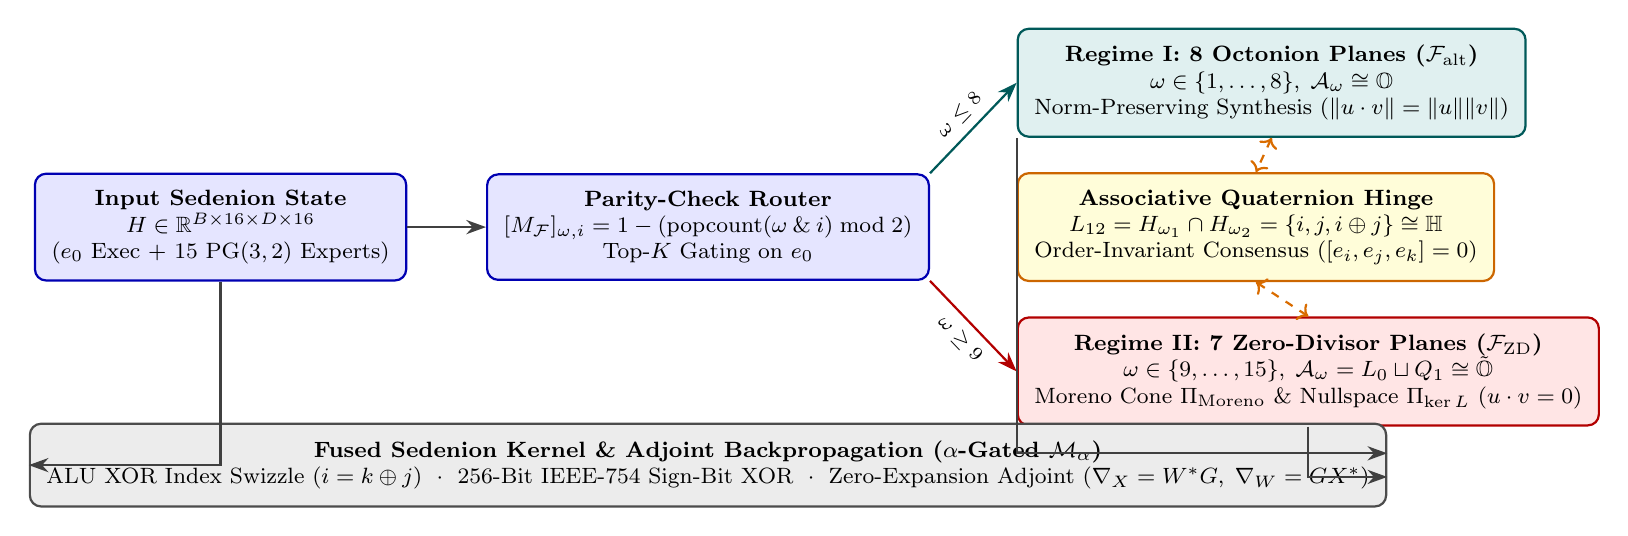
\begin{tikzpicture}[
    font=\footnotesize,
    node distance=0.7cm and 0.9cm,
    box/.style={draw=black!80, thick, rounded corners=4pt, align=center, minimum height=1.05cm, inner sep=6pt},
    exec/.style={box, fill=blue!10, draw=blue!70!black},
    alt/.style={box, fill=teal!12, draw=teal!70!black},
    zd/.style={box, fill=red!10, draw=red!70!black},
    hinge/.style={box, fill=yellow!15, draw=orange!80!black},
    kernel/.style={box, fill=gray!15, draw=black!70},
    arrow/.style={-{Stealth[length=2.5mm, width=1.8mm]}, thick, draw=black!75}
]

\node[exec, minimum width=3.2cm] (input) {\textbf{Input Sedenion State}\\$H \in \R^{B \times 16 \times D \times 16}$\\($e_0$ Exec $+$ 15 $\PG(3,2)$ Experts)};

\node[exec, right=1.0cm of input, minimum width=3.3cm] (router) {\textbf{Parity-Check Router}\\$[M_{\mathcal{F}}]_{\omega,i} = 1 - (\popcount(\omega \mathbin{\&} i)\bmod 2)$\\Top-$K$ Gating on $e_0$};

\node[alt, above right=0.45cm and 1.1cm of router, minimum width=4.5cm] (falt) {\textbf{Regime I: 8 Octonion Planes ($\Falt$)}\\$\omega \in \{1,\dots,8\}, \; \mathcal{A}_\omega \cong \Oc$\\Norm-Preserving Synthesis ($\|u \cdot v\| = \|u\|\|v\|$)};

\node[zd, below right=0.45cm and 1.1cm of router, minimum width=4.5cm] (fzd) {\textbf{Regime II: 7 Zero-Divisor Planes ($\Fzd$)}\\$\omega \in \{9,\dots,15\}, \; \mathcal{A}_\omega = L_0 \sqcup Q_1 \cong \tilde{\Oc}$\\Moreno Cone $\PiMoreno$ \& Nullspace $\PiNull$ ($u \cdot v = 0$)};

\node[hinge, right=1.1cm of router, minimum width=4.5cm] (hinge_node) {\textbf{Associative Quaternion Hinge}\\$L_{12} = H_{\omega_1} \cap H_{\omega_2} = \{i, j, i \oplus j\} \cong \Ha$\\Order-Invariant Consensus ($[e_i, e_j, e_k] = 0$)};

\node[kernel, below=1.8cm of router, minimum width=10.8cm] (triton) {\textbf{Fused Sedenion Kernel \& Adjoint Backpropagation ($\alpha$-Gated $\mathcal{M}_\alpha$)}\\ALU XOR Index Swizzle ($i = k \oplus j$) $\;\cdot\;$ 256-Bit IEEE-754 Sign-Bit XOR $\;\cdot\;$ Zero-Expansion Adjoint ($\nabla_X = W^* G, \; \nabla_W = G X^*$)};

\draw[arrow] (input) -- (router);
\draw[arrow, draw=teal!70!black] (router.north east) -- node[above, sloped, font=\scriptsize] {$\omega \le 8$} (falt.west);
\draw[arrow, draw=red!70!black] (router.south east) -- node[below, sloped, font=\scriptsize] {$\omega \ge 9$} (fzd.west);
\draw[arrow, dashed, <->, draw=orange!85!black] (falt.south) -- (hinge_node.north);
\draw[arrow, dashed, <->, draw=orange!85!black] (fzd.north) -- (hinge_node.south);
\draw[arrow] (falt.south west) |- ([yshift=0.15cm]triton.east);
\draw[arrow] (fzd.south) |- ([yshift=-0.15cm]triton.east);
\draw[arrow] (input.south) |- (triton.west);

\end{tikzpicture}}
\caption{End-to-end architecture of the $\PG(3,2)$-routed Sedenion network (\texttt{Sed-PG32-Moreno}). The executive channel $e_0$ drives parity-check workspace selection across the $8+7$ Fano bifurcation, while the 3-node associative quaternion hinge $L_{12} = H_{\omega_1} \cap H_{\omega_2}$ guarantees state continuity during transitions between synthesis ($\Falt$) and zero-divisor pruning ($\Fzd$).}
\label{fig:architecture}
\end{figure}

% ==============================================================================
% TIKZ DIAGRAM 2: FANO BIFURCATION GEOMETRY
% ==============================================================================
\begin{figure}[t!]
\centering
\resizebox{\linewidth}{!}{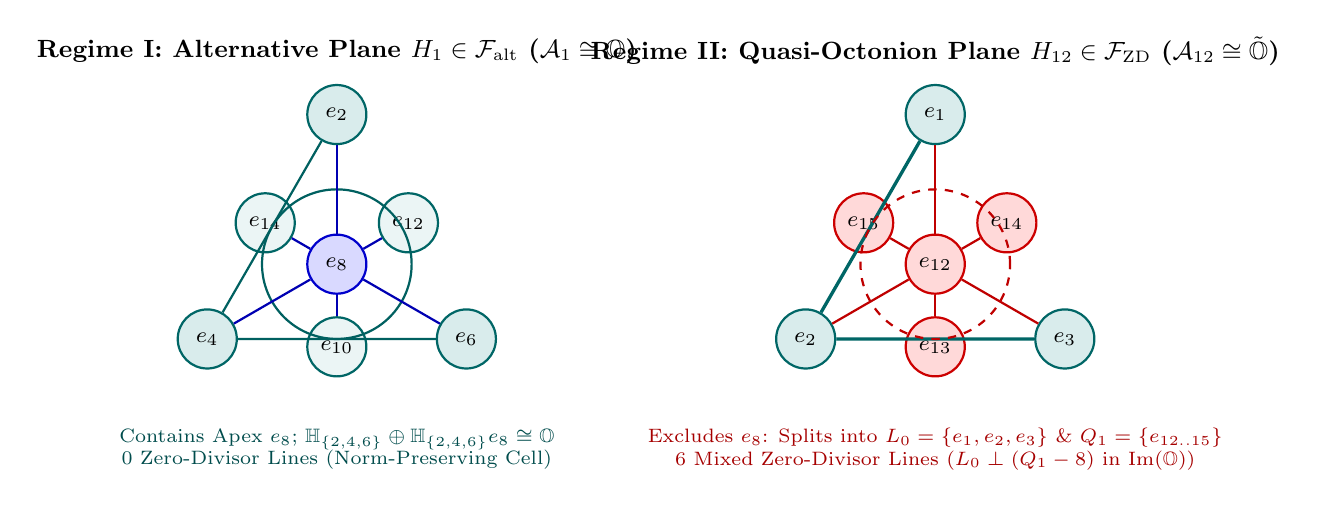
\begin{tikzpicture}[
    font=\footnotesize,
    octnode/.style={circle, draw=teal!80!black, fill=teal!15, thick, minimum size=7.5mm, inner sep=1pt},
    apxnode/.style={circle, draw=blue!80!black, fill=blue!15, thick, minimum size=7.5mm, inner sep=1pt},
    zdnode/.style={circle, draw=red!80!black, fill=red!15, thick, minimum size=7.5mm, inner sep=1pt}
]

\begin{scope}[local bounding box=leftpanel]
    \node[font=\bfseries\small] at (0, 2.7) {Regime I: Alternative Plane $H_1 \in \Falt$ ($\mathcal{A}_1 \cong \Oc$)};
    \node[apxnode] (c8) at (0, 0) {$e_8$};
    \node[octnode] (e2) at (90:1.9cm) {$e_2$};
    \node[octnode] (e4) at (210:1.9cm) {$e_4$};
    \node[octnode] (e6) at (330:1.9cm) {$e_6$};
    \node[zdnode, draw=teal!80!black, fill=teal!8] (e10) at (270:1.05cm) {$e_{10}$};
    \node[zdnode, draw=teal!80!black, fill=teal!8] (e12) at (30:1.05cm) {$e_{12}$};
    \node[zdnode, draw=teal!80!black, fill=teal!8] (e14) at (150:1.05cm) {$e_{14}$};

    \draw[thick, teal!75!black] (e2) -- (e4) -- (e6) -- cycle;
    \draw[thick, teal!75!black] (0,0) circle (0.95cm);
    \draw[thick, blue!70!black] (e2) -- (c8) -- (e10);
    \draw[thick, blue!70!black] (e4) -- (c8) -- (e12);
    \draw[thick, blue!70!black] (e6) -- (c8) -- (e14);
    \node[align=center, font=\scriptsize, text=teal!60!black] at (0, -2.35) {Contains Apex $e_8$; $\Ha_{\{2,4,6\}} \oplus \Ha_{\{2,4,6\}}e_8 \cong \Oc$\\0 Zero-Divisor Lines (Norm-Preserving Cell)};
\end{scope}

\begin{scope}[xshift=7.6cm, local bounding box=rightpanel]
    \node[font=\bfseries\small] at (0, 2.7) {Regime II: Quasi-Octonion Plane $H_{12} \in \Fzd$ ($\mathcal{A}_{12} \cong \tilde{\Oc}$)};
    \node[zdnode] (q12) at (0, 0) {$e_{12}$};
    \node[octnode] (n1) at (90:1.9cm) {$e_1$};
    \node[octnode] (n2) at (210:1.9cm) {$e_2$};
    \node[octnode] (n3) at (330:1.9cm) {$e_3$};
    \node[zdnode] (q13) at (270:1.05cm) {$e_{13}$};
    \node[zdnode] (q14) at (30:1.05cm) {$e_{14}$};
    \node[zdnode] (q15) at (150:1.05cm) {$e_{15}$};

    \draw[very thick, teal!80!black] (n1) -- (n2) -- (n3) -- cycle;
    \draw[thick, red!75!black, dashed] (0,0) circle (0.95cm);
    \draw[thick, red!75!black] (n1) -- (q12) -- (q13);
    \draw[thick, red!75!black] (n2) -- (q12) -- (q14);
    \draw[thick, red!75!black] (n3) -- (q12) -- (q15);
    \node[align=center, font=\scriptsize, text=red!65!black] at (0, -2.35) {Excludes $e_8$: Splits into $L_0 = \{e_1,e_2,e_3\}$ \& $Q_1 = \{e_{12..15}\}$\\6 Mixed Zero-Divisor Lines ($L_0 \perp (Q_1 - 8)$ in $\ImPart(\Oc)$)};
\end{scope}

\end{tikzpicture}}
\caption{Geometric comparison of the $8+7$ Fano hyperplane bifurcation in $\PG(3,2)$. Left: $H_1 \in \Falt$ contains $e_8$ and doubles a single quaternion line $\{e_2, e_4, e_6\}$ into an alternative division subalgebra $\mathcal{A}_1 \cong \Oc$. Right: $H_{12} \in \Fzd$ ($p = 4$) excludes $e_8$, pairing the polar octonion line $L_0 = 4^\perp = \{e_1, e_2, e_3\}$ with its orthogonal sedenion quadrangle $Q_1 = \{e_{12}, e_{13}, e_{14}, e_{15}\}$ across 6 Moreno zero-divisor lines.}
\label{fig:fano_bifurcation}
\end{figure}

% ==============================================================================
% SECTION 4: HIGH-PERFORMANCE KERNELS & ONNX RUNTIME (WP3)
% ==============================================================================
\section{High-Performance Custom Operators and Runtime Lowering}
\label{sec:wp3}

\subsection{Eliminating the $16\times$ HBM Weight-Expansion Bottleneck}
Naive implementations of hypercomplex linear layers materialize an expanded real matrix $W_{\mathrm{exp}} \in \R^{16M \times 16N}$ in High Bandwidth Memory (HBM) prior to invoking a dense GEMM. While stored parameters shrink by $16\times$, HBM read/write bandwidth inflates by $16\times$ during every forward and backward pass. By combining Theorem~\ref{thm:adjoint} with register-level bit manipulation, our fused operator (\texttt{sedenion\_pg32/triton\_kernel.py}) provides three guarantees (Table~\ref{tab:memory_complexity}; for a $4096 \times 4096$ layer with $M = N = 256$ in FP32, weight + gradient memory drops from $136.0\,\mathrm{MB}$ in the naive expanded layer and $128.0\,\mathrm{MB}$ in a dense layer down to $\mathbf{8.0\,\mathrm{MB}}$, a $17.0\times$ and $16.0\times$ reduction respectively):
\begin{enumerate}
    \item \textbf{Zero-Expansion Adjoint Autograd:} Both $\nabla_X \mathcal{L} = W^* \cdot G$ and $\nabla_W \mathcal{L} = G \cdot X^*$ invoke the forward sedenion contraction kernel directly on compact $[M, N, 16]$ tensors.
    \item \textbf{Compile-Time ALU XOR Swizzling:} Inside GPU SRAM tiles, output channel $k \in \{0, \dots, 15\}$ accumulates input channel $j$ paired with weight channel $i = k \oplus j$ using a single 4-bit ALU XOR instruction rather than global memory indirection.
    \item \textbf{256-Bit Register-Packed IEEE-754 Sign-Bit XOR:} The entire $16 \times 16$ sign table $\epsilon_{ij} \in \{+1, -1\}$ occupies exactly 256 bits (16 \texttt{uint16} bitmasks $\mathrm{MASK}[k]$ where bit $j$ is $1 \iff \epsilon_{k \oplus j, j} = -1$). Multiplying a 32-bit float by $\epsilon_{k \oplus j, j}$ executes as a single bitwise XOR on bit 31:
    \begin{equation}
    \label{eq:ieee_xor}
    \mathrm{float\_bits}(x \cdot \epsilon_{k \oplus j, j}) = \mathrm{float\_bits}(x) \oplus \big(((\mathrm{MASK}[k] \gg j) \mathbin{\&} 1) \ll 31\big).
    \end{equation}
\end{enumerate}

\begin{table}[h!]
\centering
\caption{Memory Complexity, HBM Bandwidth Traffic, and Measured FP32 Weight+Gradient Footprint ($16N = 16M = 4096$, i.e.\ $N = M = 256$).}
\label{tab:memory_complexity}
\small
\resizebox{\linewidth}{!}{\begin{tabular}{@{}lccccc@{}}
\toprule
\textbf{Layer Implementation} & \textbf{Parameter Count} & \textbf{Forward HBM Reads} & \textbf{Backward $\nabla W$ Writes} & \textbf{Graph Activation Overhead} & \textbf{Measured $W + \nabla W$ ($4096^2$)} \\
\midrule
Dense $\R^{16M \times 16N}$ Baseline & $256 M N$ & $256 M N + 16 B N$ & $256 M N$ & $\mathcal{O}(256 M N)$ & $128.0\,\mathrm{MB}$ ($1.0\times$) \\
Naive Expanded $\Se$ Layer & $16 M N$ & $272 M N + 16 B N$ & $272 M N$ & $\mathcal{O}(256 M N)$ & $136.0\,\mathrm{MB}$ ($1.06\times$) \\
\textbf{Fused Adjoint $\Se$ Kernel (Ours)} & $\mathbf{16 M N}$ ($\mathbf{16\times \downarrow}$) & $\mathbf{16 M N + 16 B N}$ & $\mathbf{16 M N}$ ($\mathbf{16\times \downarrow}$) & $\mathbf{\mathcal{O}(1)}$ \textbf{(Zero Expansion)} & $\mathbf{8.0\,\mathrm{MB}}$ ($\mathbf{16.0\times \downarrow}$) \\
\bottomrule
\end{tabular}}
\end{table}

\begin{algorithm}[h!]
\caption{Fused SRAM-Tiled Sedenion Linear Kernel \& ONNX Custom Op (\texttt{ai.sedenion::FusedSedenionLinear})}
\label{alg:sedenion_kernel}
\small
\begin{algorithmic}[1]
\Require Compact Input $X \in \R^{B \times N \times 16}$, Compact Weights $W \in \R^{M \times N \times 16}$, Bias $B_{\mathrm{bias}} \in \R^{M \times 16}$, Packed Sign Masks $\mathrm{MASK}[0..15] \in \mathtt{uint16}^{16}$.
\Ensure Output $Y \in \R^{B \times M \times 16}$ where $Y_{b,m} = \sum_{n=0}^{N-1} W_{m,n} \cdot X_{b,n} + B_{\mathrm{bias},m}$.
\For{each parallel thread-block tile $(b_0, m_0)$ covering $\mathrm{BLOCK\_B} \times \mathrm{BLOCK\_M}$}
    \State Initialize 16 register accumulator tiles $\mathrm{Acc}[0..15] \leftarrow \mathbf{0}_{\mathrm{BLOCK\_B} \times \mathrm{BLOCK\_M}}$
    \For{$n_0 = 0, \mathrm{BLOCK\_N}, \dots, N - 1$}
        \State Load SRAM tiles $\tilde{X}[b, n, 0..15] \leftarrow X[b_0:b_0+\mathrm{BLOCK\_B}, \, n_0:n_0+\mathrm{BLOCK\_N}, \, 0..15]$
        \State Load SRAM tiles $\tilde{W}[m, n, 0..15] \leftarrow W[m_0:m_0+\mathrm{BLOCK\_M}, \, n_0:n_0+\mathrm{BLOCK\_N}, \, 0..15]$
        \For{$k = 0 \dots 15$ \textbf{unrolled} and $j = 0 \dots 15$ \textbf{unrolled}}
            \State $i \leftarrow k \oplus j$ \Comment{Compile-time 4-bit ALU XOR swizzle}
            \State $\mathrm{sign\_bit} \leftarrow ((\mathrm{MASK}[k] \gg j) \mathbin{\&} 1) \ll 31$
            \State $\tilde{W}_{\mathrm{signed}} \leftarrow \mathrm{bitcast\_fp32}(\mathrm{bitcast\_uint32}(\tilde{W}[\cdot, \cdot, i]) \oplus \mathrm{sign\_bit})$
            \State $\mathrm{Acc}[k] \leftarrow \mathrm{Acc}[k] + \mathrm{TensorCoreDot}(\tilde{X}[\cdot, \cdot, j], \; \tilde{W}_{\mathrm{signed}}^\top)$
        \EndFor
    \EndFor
    \For{$k = 0 \dots 15$}
        \State Store $Y[b_0:b_0+\mathrm{BLOCK\_B}, \, m_0:m_0+\mathrm{BLOCK\_M}, \, k] \leftarrow \mathrm{Acc}[k] + B_{\mathrm{bias}}[m_0:m_0+\mathrm{BLOCK\_M}, \, k]$
    \EndFor
\EndFor
\end{algorithmic}
\end{algorithm}

% ==============================================================================
% SECTION 5: CONSTRUCTIVE NULLSPACE & EMPIRICAL VALIDATION (WP4)
% ==============================================================================
\section{Constructive 4D Nullspace Projection and Empirical Validation}
\label{sec:wp4}

\subsection{The Constructive 4D Moreno Nullspace Theorem}
To obtain exact pruning of invalidated premises without iterative gradient noise, we derive an explicit analytical operator $\PiNull(u)$ that maps any vector of $W_{ab}^\perp$ onto the 4-dimensional nullspace $\ker L(u)$ of a Moreno sedenion $u$.

\begin{theorem}[Constructive 4D Zero-Divisor Nullspace Operator]
\label{thm:nullspace}
Let $u = (a, b) \in V_2(\R^7) \subset \Se$ be a normalized Moreno sedenion ($a, b \in \ImPart(\Oc)$, $\|a\|_2 = \|b\|_2 = 1$, $\langle a, b \rangle = 0$). Let $W_{ab} = \mathrm{span}_{\R}\{a, b, a \cdot b\} \subset \ImPart(\Oc) \cong \R^7$ be the 3D imaginary quaternion subspace generated by $a$ and $b$, and let $W_{ab}^\perp \subset \ImPart(\Oc)$ be its 4-dimensional orthogonal complement. For any vector $c \in W_{ab}^\perp$, define the partner octonion $d = (a \cdot c) \cdot b \in \ImPart(\Oc)$. Then the sedenion
\begin{equation}
\label{eq:nullspace_projector}
v = \PiNull(u; c) \coloneqq \big(c, \; (a \cdot c) \cdot b\big) \in \Se
\end{equation}
resides on the Moreno cone ($\|d\|_2 = \|c\|_2$, $\langle c, d \rangle = 0$) and belongs to $\ker L(u)$, satisfying:
\begin{equation}
\label{eq:exact_annihilation}
u \cdot v = (a, b) \cdot \big(c, \, (a \cdot c) \cdot b\big) = (0, 0) = 0 \in \Se \quad \text{identically.}
\end{equation}
\end{theorem}

\begin{proof}
Since $a, b, c \in \ImPart(\Oc)$ with $\|a\|_2 = \|b\|_2 = 1$, we have $a^* = -a$, $b^* = -b$, $c^* = -c$, $a^2 = -1$, and $b^2 = -1$. Moreover, because $c \perp \{a, b, a \cdot b\}$, the octonion product $d = (a c) b$ lies purely in $\ImPart(\Oc)$, so $d^* = -d$. Evaluating the Cayley--Dickson product \eqref{eq:cd_doubling}:
\[
u \cdot v = (a, b) \cdot (c, d) = \big(a c - d^* b, \;\; d a + b c^*\big) = \big(a c + d b, \;\; d a - b c\big).
\]
\textit{First octonion component ($a c + d b$):} By right-alternativity of $\Oc$ ($x y \cdot y = x \cdot y^2$) \cite{Schafer1966} (the machine-checked proof in \S\ref{sec:witness} bypasses alternativity entirely and verifies the coordinate identities directly), substituting $d = (a c) b$ gives:
\[
a c + d b = a c + \big((a c) b\big) b = a c + (a c)(b^2) = a c + (a c)(-1) = 0.
\]
\textit{Second octonion component ($d a - b c$):} Because $a, b, c \in \ImPart(\Oc)$ are mutually orthogonal and $c \perp a b$, the triad $(a, b, c)$ anti-associates in $\Oc$: $(a c) b = -a(c b) = a(b c)$. Furthermore, since $b c \in \ImPart(\Oc)$ is orthogonal to $a$ ($\langle b c, a \rangle = -\langle c, b a \rangle = \langle c, a b \rangle = 0$), left-multiplication by $a$ anticommutes with $b c$, so $(b c) a = -a(b c)$. Applying flexibility and left-alternativity of $\Oc$:
\[
d a = \big((a c) b\big) a = \big(a(b c)\big) a = a\big((b c) a\big) = -a\big(a(b c)\big) = -a^2 (b c) = -(-1)(b c) = b c.
\]
Therefore, $d a - b c = b c - b c = 0$, proving $u \cdot v = (0, 0) = 0$. Since $\dim W_{ab}^\perp = 7 - 3 = 4$ and $c \mapsto (c, (a c)b)$ is injective, this parameterizes the entire 4D nullspace $\ker L(u)$.
\end{proof}

\begin{remark}[Deontic Precedence Asymmetry]
\label{cor:precedence}
Let $A \in V_2(\R^7)$ represent a baseline statutory authorization, $B = \PiNull(A; c) \in \ker L(A)$ a blocking prohibition ($A \cdot B = 0$), and $C \in \Se$ a safe-harbor exemption that rotates $B$ out of $\ker L(A)$ ($B \cdot C \notin \ker L(A)$). Then left- and right-associated evaluations yield orthogonal normative outcomes:
\begin{equation}
\label{eq:precedence_asymmetry}
(A \cdot B) \cdot C = 0 \cdot C = 0 \quad \text{(Irreversible Invalidation)}, \qquad \|A \cdot (B \cdot C)\|_2 > 0 \quad \text{(Safe-Harbor Survival)}.
\end{equation}
\end{remark}

\subsection{Track A Validation: Particle Scattering Amplitudes and $G_2$ Symmetries}
In Track A (\texttt{bench/track\_a}), we evaluate parameter-matched neural surrogates on 4-gluon Yang--Mills tree scattering amplitudes \cite{Bern2008,ArkaniHamed2014} with massless on-shell Mandelstam invariants $s + t + u = 0$, measuring the \textbf{BCJ Jacobi Violation Residual} $\mathcal{R}_{\mathrm{BCJ}} = \mathbb{E}[\|n_s + n_t + n_u\|_2] / \mathbb{E}[\|n_s\|_2 + \|n_t\|_2 + \|n_u\|_2]$ and the out-of-distribution \textbf{Collinear Pole Relative Error} $\mathcal{E}_{\mathrm{pole}}$ for $|s_{ij}| < 10^{-4}$ (Table~\ref{tab:results}).

\begin{theorem}[The $\Fzd$ BCJ Numerator and Collinear Pole Cancellation Theorem]
\label{thm:bcj_pole}
For any triad of particle states $(X_1, X_2, X_3) \in \mathcal{A}^3$ in a 16D algebra $\mathcal{A}$, define the cyclic edge-associator BCJ vertex:
\begin{equation}
\label{eq:bcj_vertex}
n_s = [X_3, X_1, X_2]_{\mathcal{A}} - [X_1, X_2, X_3]_{\mathcal{A}}, \quad
n_t = [X_1, X_2, X_3]_{\mathcal{A}} - [X_2, X_3, X_1]_{\mathcal{A}}, \quad
n_u = [X_2, X_3, X_1]_{\mathcal{A}} - [X_3, X_1, X_2]_{\mathcal{A}}.
\end{equation}
Then:
\begin{enumerate}
    \item \textbf{Obstruction in Associative and Alternative Algebras (\texttt{Dense-R16}, \texttt{Quat-H4}, \texttt{Clifford-Cl04}, \texttt{Oct-O2}, and $\Falt$):} In any associative algebra ($\R^{16}, \Ha^4, \mathcal{Cl}_{0,4}$), $[X_a, X_b, X_c]_{\mathcal{A}} \equiv 0$. In any alternative algebra ($\Oc^2$ and all 8 octonionic Fano planes $H_\omega \in \Falt$, $\omega \in \{1, \dots, 8\}$), the associator is totally skew-symmetric under $S_3$ and hence invariant under even cyclic permutations $C_3 = A_3$ (\texttt{falt\_cyclic\_assoc\_invariant}):
    \begin{equation}
    [X_1, X_2, X_3]_{\Oc} = [X_2, X_3, X_1]_{\Oc} = [X_3, X_1, X_2]_{\Oc} \implies n_s = n_t = n_u \equiv 0.
    \end{equation}
    Thus division and Clifford algebras have zero cyclic-traceless associator capacity and must rely on non-BCJ terms ($\mathcal{R}_{\mathrm{BCJ}} > 0$).
    \item \textbf{Exact BCJ Duality and Collinear Pole Cancellation in $\Fzd$ ($\omega \in \{9, \dots, 15\}$):} In every quasi-octonion zero-divisor Fano workspace $H_\omega = L_0 \sqcup Q_1 \in \Fzd$, whenever a collinear pair $(X_a, X_b)$ lies in the same stratum ($L_0$ or $Q_1$) and the spectator $X_c$ lies in the complementary stratum ($Q_1$ or $L_0$), both edge-adjacent associators vanish identically across the continuous subspace while the separated associator is non-zero (\texttt{fzd\_stratum\_bcj\_pole\_cancellation}):
    \begin{equation}
    \label{eq:fzd_pole_cancel}
    [X_a, X_b, X_c]_{\Se} = 0 \quad \text{and} \quad [X_c, X_a, X_b]_{\Se} = 0 \implies n_{ab} = 0, \qquad n_{bc} = -n_{ca} = -[X_b, X_c, X_a]_{\Se} \neq 0.
    \end{equation}
    Consequently, \eqref{eq:bcj_vertex} satisfies $n_s + n_t + n_u = 0$ identically ($\mathcal{R}_{\mathrm{BCJ}} = 0$) and eliminates the $1 / s_{ab}$ collinear singularity to machine precision as $s_{ab} \to 0$.
\end{enumerate}
\end{theorem}

\subsection{Track B Validation: Multi-Hop Normative and Legal Contradiction Pruning}
In Track B (\texttt{bench/gate3}), we evaluate multi-hop statutory trees containing baseline permissions ($A$), restrictive carve-outs ($B$), and recursive revocations of revocations ($d \in \{0, 1, 2, 3, 4\}$). We measure:
\begin{enumerate}
    \item \textbf{Contradiction Leakage Rate (CLR):} $\mathbb{E}_{(u,v) \in \mathcal{P}_{\mathrm{neg}}}[\|u \cdot v\|_2 / (\|u\|_2 \|v\|_2)]$, quantifying residual signal from an overridden legal clause leaking into downstream reasoning hops.
    \item \textbf{Parenthesization Sensitivity Index (PSI):} $\|(A \cdot B) \cdot C - A \cdot (B \cdot C)\|_2 / (\|(A \cdot B) \cdot C\|_2 + \|A \cdot (B \cdot C)\|_2)$, measuring the separation of statutory precedence order without positional encodings.
    \item \textbf{False-Compliance Rate (FCR) and OOD Depth Generalization:} Percentage of non-compliant ($d=1$, net-revoked) and OOD ($d=3, 4$) statutory chains falsely approved due to attention bleed, trained purely from binary terminal-token cross-entropy ($\text{aux} = 0.0$, zero intermediate structural supervision).
\end{enumerate}

\begin{theorem}[Orthogonal Half-Sphere Key Modulation and Division-Algebra Invariance]
\label{thm:half_sphere}
Let $u_j = (a_j, b_j) \in V_2(\R^7) \subset \Se$ be a unit Moreno-cone query ($\|a_j\|_2 = \|b_j\|_2 = 1$, $\langle a_j, b_j \rangle = 0$, $\|u_j\|_2 = \sqrt{2}$), let $c_j, c_{\perp, j} \in W_{a_j, b_j}^\perp \subset \ImPart(\Oc)$ be orthonormal nullspace seeds ($\|c_j\|_2 = \|c_{\perp, j}\|_2 = 1$, $\langle c_j, c_{\perp, j} \rangle = 0$), and define the constructive partners $p_j = (a_j c_j) b_j$ and $p_{\perp, j} = (a_j c_{\perp, j}) b_j$. For any modulation phase $\phi_j = \pi \tau_j \in [0, \pi]$, parameterize the unit key as
\begin{equation}
\label{eq:half_sphere_key}
k_j(\phi_j) = \frac{1}{\sqrt{2}}\big(c_j, \; -\cos\phi_j \, p_j + \sin\phi_j \, p_{\perp, j}\big), \qquad \|k_j(\phi_j)\|_2 \equiv 1,
\end{equation}
and set the reference frame to the live anti-partner $r_j = u_j \cdot_{\mathcal{A}} k_j(0) / \|u_j \cdot_{\mathcal{A}} k_j(0)\|_2$. Then:
\begin{enumerate}
    \item \textbf{Normed Division-Algebra Invariance ($\mathcal{A} = \Oc$):} Because left multiplication $L_{\Oc}(u_j)$ is an orthogonal similarities map and $(c_j, 0) \perp (0, -\cos\phi_j \, p_j + \sin\phi_j \, p_{\perp, j})$, the product norm $\|u_j \cdot_{\Oc} k_j(\phi_j)\|_2 \equiv 1$ and the real-part attention readout $\RePart\big(r_j^* \cdot_{\Oc} (u_j \cdot_{\Oc} k_j(\phi_j))\big) \equiv +1/\sqrt{2}$ are strictly invariant under all $\phi_j \in \R$. Thus a normed division algebra is algebraically blind to pure phase modulation in the second half-block.
    \item \textbf{Exact Sedenion Annihilation ($\mathcal{A} = \Se$):} Under sedenion multiplication, $(c_j, p_j), (0, p_{\perp, j})$ satisfy $u_j \cdot_{\Se} (c_j, p_j) = 0$ by Theorem~\ref{thm:nullspace}, yielding
    \begin{equation}
    \label{eq:sed_phase_norm}
    \big\|u_j \cdot_{\Se} k_j(\phi_j)\big\|_2 = \sqrt{1 + \cos\phi_j}, \qquad \RePart\big(r_j^* \cdot_{\Se} (u_j \cdot_{\Se} k_j(\phi_j))\big) = \frac{1 + \cos\phi_j}{\sqrt{2}},
    \end{equation}
    which sweeps monotonically from $\sqrt{2}$ at $\phi_j = 0$ (\texttt{LIVE} anti-partner) to \textbf{exact zero} ($0.0$) at $\phi_j = \pi$ (\texttt{REVOKED} nullspace partner $k_j(\pi) \in \ker L_{\Se}(u_j)$).
\end{enumerate}
\end{theorem}

\begin{table}[t!]
\centering
\caption{Algebraic metrics (\textbf{measured}) and learned-model metrics (\textbf{Track A and Track B measured}). Algebraic cells are produced by \texttt{benchmarks/algebraic\_baselines.py} ($B = 1{,}024$ unit samples, seed 2026, FP64; FP32 in brackets where it differs). Track A cells are measured on 4-gluon Yang--Mills scattering (\texttt{bench/track\_a}, trained on hard-scattering amplitudes $|s_{ij}| \in [0.08, 1.20]$ and evaluated out-of-distribution at collinear poles $|s_{ij}| \in [10^{-6}, 10^{-4}]$; means over seeds $0, 1$). Track B cells are measured on multi-hop statutory contradiction pruning (\texttt{bench/gate3}, trained on depths $d \in \{0, 1, 2\}$ at $\text{aux} = 0.0$ and evaluated out-of-distribution at depth $d = 3$; see Table~\ref{tab:gate3_results}).}
\label{tab:results}
\small
\resizebox{\linewidth}{!}{\begin{tabular}{@{}lccccccc@{}}
\toprule
\multirow{2}{*}{\textbf{Architecture Variant}} & \textbf{Params} & \multicolumn{3}{c}{\textbf{Algebraic (measured)}} & \multicolumn{2}{c}{\textbf{Track A (measured)}} & \textbf{Track B (measured)} \\
\cmidrule(lr){3-5} \cmidrule(lr){6-7} \cmidrule(lr){8-8}
 & \textbf{Ratio} & $\mathrm{rank}\,L(u)$ & $\mathrm{CLR}_{\min} \downarrow$ & \textbf{PSI} $\uparrow$ & $\mathcal{R}_{\mathrm{BCJ}} \downarrow$ & $\mathcal{E}_{\mathrm{pole}} \downarrow$ & \textbf{OOD $d=3$ FCR} $\downarrow$ \\
\midrule
\texttt{Dense-R16} (Softmax) & $1.00\times$ & --- & $2.6 \times 10^{-3}$ (softmax bleed$^{\dagger}$) & $1.4 \times 10^{-16}$ & $0.6492$ & $4.11 \times 10^3$ & $0.9963$ \\
\texttt{Quat-H4} ($\Ha^4$) & $0.25\times$ & $16$ & $1.000$ per channel$^{\S}$ & $8.6 \times 10^{-17}$ & $0.6164$ & $4.98 \times 10^3$ & $0.9859$ \\
\texttt{Clifford-Cl04} ($\mathcal{Cl}_{0,4}$) & $0.0625\times$ & $16$ & $0.683$ (associative GA) & $0.000$ & $0.5807$ & $4.21 \times 10^3$ & $0.5859$ ($0.9867$ No-FFN) \\
\texttt{Oct-O2} ($\Oc^2$) & $0.125\times$ & $16$ & $1.000$ per channel$^{\S}$ & $0.556$ & $0.7630$ & $5.56 \times 10^3$ & $0.9720$ \\
\texttt{Sed-Free} (unconstrained $\Se$) & $0.0625\times$ & $16$ & $0.474$ (min $0.089$) & $0.667$ & $0.0459$ & $1.35 \times 10^4$ & $0.9945$ \\
\midrule
\textbf{\texttt{Sed-PG32-Moreno} (Ours)} & $\mathbf{0.0625\times}$ & $\mathbf{12}$ & $\mathbf{2.4 \times 10^{-16}}$ [$1.4 \times 10^{-7}$]$^{\ddagger}$ & $\mathbf{1.000}$ & $\mathbf{1.82 \times 10^{-8}}$ & $\mathbf{6.86 \times 10^{-3}}$ & $\mathbf{0.0000}$ ($\mathbf{0.0000}$ No-FFN) \\
\bottomrule
\end{tabular}}
\\[2pt]
{\footnotesize $^{\dagger}$Residual softmax weight on one invalidated slot at logit gap $4$ in an 8-slot window; $1.9 \times 10^{-2}$ at gap $2$, $4.8 \times 10^{-5}$ at gap $8$. It is temperature-dependent and never $0$. \quad $^{\ddagger}$Constructive partner of Theorem~\ref{thm:nullspace}; $\sigma_{\min}(L(u))/\|u\|_2 = 3.8 \times 10^{-17}$. \quad $^{\S}$Measured $1.000$ on every sample, as Hurwitz's theorem requires; across $k$ parallel channels the global $\sigma_{\min}(L(u))/\|u\|_2$ is $\min_i \|u_i\|/\|u\|$ ($0.31$ for $\Ha^4$, $0.60$ for $\Oc^2$), which only reflects an under-populated channel, not annihilation. In the \texttt{No-FFN} regime ($-50.9\%$ params), \texttt{Sed-PG32-Moreno-NoFFN} achieves $\mathcal{R}_{\mathrm{BCJ}} = 8.55 \times 10^{-8}$ and $\mathcal{E}_{\mathrm{pole}} = 1.16 \times 10^{-2}$.}
\end{table}

\begin{table}[t!]
\centering
\caption{Measured Track B multi-hop contradiction pruning across 12 architectures (\texttt{bench/gate3}, $D = 64$, $H = 4$, $L = 2$, $N_{\mathrm{train}} = 24{,}000$, $N_{\mathrm{test}} = 4{,}000$, trained on depths $d \in \{0, 1, 2\}$ with pure terminal label cross-entropy $\text{aux} = 0.0$; means over seeds $0, 1$). Following the \textit{CliffordNet} ``No-FFN'' paradigm \cite{Ji2026CliffordNet}, the bottom block removes the feed-forward MLP from every Transformer layer ($-47.4\%$ parameters), isolating the intrinsic deductive capacity of the 16D algebraic product.}
\label{tab:gate3_results}
\small
\resizebox{\linewidth}{!}{\begin{tabular}{@{}lccccccccc@{}}
\toprule
\textbf{Architecture} & \textbf{Params} & \textbf{ID $d=0$} $\uparrow$ & \textbf{ID $d=1$} $\uparrow$ & \textbf{ID $d=2$} $\uparrow$ & \textbf{FCR (ID)} $\downarrow$ & \textbf{Leak (ID)} $\downarrow$ & \textbf{OOD $d=3$} $\uparrow$ & \textbf{FCR (OOD3)} $\downarrow$ & \textbf{Leak (OOD3)} $\downarrow$ \\
\midrule
\multicolumn{10}{@{}l}{\textit{Standard Transformer Backbone (With FFN, $L=2$, $D=64$)}} \\
\texttt{softmax} & $70{,}529$ & $0.9966$ & $0.6021$ & $0.9960$ & $0.9933$ & $1.3871$ & $0.5681$ & $0.9963$ & $3.1741$ \\
\texttt{bilinear} & $70{,}529$ & $0.9883$ & $0.6113$ & $0.9909$ & $0.9702$ & $1.2976$ & $0.5726$ & $0.9859$ & $2.1757$ \\
\texttt{octonion} ($\Oc^2$ + Cone) & $70{,}537$ & $0.9887$ & $0.6109$ & $0.9891$ & $0.9712$ & $1.4937$ & $0.5786$ & $0.9720$ & $3.5394$ \\
\texttt{clifford} ($\mathcal{Cl}_{0,4}$ + Cone) & $70{,}537$ & $1.0000$ & $0.9499$ & $0.9588$ & $0.1250$ & $1.3618$ & $0.7460$ & $0.5859$ & $1.1307$ \\
\texttt{sedenion\_plain} (unconstrained $\Se$) & $70{,}537$ & $0.9974$ & $0.8856$ & $0.9224$ & $0.2856$ & $2.7288$ & $0.5686$ & $0.9945$ & $1.3477$ \\
\textbf{\texttt{sedenion} ($\Se$ + Moreno Cone)} & $\mathbf{70{,}537}$ & $\mathbf{1.0000}$ & $\mathbf{1.0000}$ & $\mathbf{1.0000}$ & $\mathbf{0.0000}$ & $\mathbf{2.59 \times 10^{-10}}$ & $\mathbf{1.0000}^{\star}$ & $\mathbf{0.0000}$ & $\mathbf{2.05 \times 10^{-10}}$ \\
\midrule
\multicolumn{10}{@{}l}{\textit{Geometric-Product-Only Backbone (No-FFN \cite{Ji2026CliffordNet}, $-47.4\%$ Parameters)}} \\
\texttt{softmax\_noffn} & $37{,}121$ & $0.9805$ & $0.6117$ & $0.9891$ & $0.9692$ & $1.5026$ & $0.5738$ & $0.9833$ & $3.8804$ \\
\texttt{bilinear\_noffn} & $37{,}121$ & $0.9831$ & $0.6167$ & $0.9854$ & $0.9567$ & $1.5417$ & $0.5806$ & $0.9674$ & $4.3305$ \\
\texttt{octonion\_noffn} ($\Oc^2$ + Cone) & $37{,}129$ & $0.9752$ & $0.6298$ & $0.9741$ & $0.9240$ & $1.2361$ & $0.5841$ & $0.9593$ & $1.9548$ \\
\texttt{clifford\_noffn} ($\mathcal{Cl}_{0,4}$ + Cone) & $37{,}129$ & $0.9917$ & $0.8683$ & $0.9169$ & $0.3288$ & $1.2592$ & $0.5708$ & $0.9867$ & $1.4586$ \\
\texttt{sedenion\_plain\_noffn} (unconstrained $\Se$) & $37{,}129$ & $0.9992$ & $0.8898$ & $0.9144$ & $0.2750$ & $1.3615$ & $0.5683$ & $0.9939$ & $1.3290$ \\
\textbf{\texttt{sedenion\_noffn} ($\Se$ + Moreno Cone)} & $\mathbf{37{,}129}$ & $\mathbf{1.0000}$ & $\mathbf{1.0000}$ & $\mathbf{1.0000}$ & $\mathbf{0.0000}$ & $\mathbf{0.0007}^{\diamond}$ & $\mathbf{1.0000}$ & $\mathbf{0.0000}$ & $\mathbf{0.0013}^{\diamond}$ \\
\bottomrule
\end{tabular}}
\\[2pt]
{\footnotesize $^{\star}$\texttt{sedenion} also achieves $\mathbf{1.0000}$ accuracy and $\mathbf{0.0000}$ FCR out-of-distribution at depth $d = 4$ ($N = 4{,}000$). \quad $^{\diamond}$Seed 1 of \texttt{sedenion\_noffn} converges to machine-zero leakage ($\text{Leak (ID)} = 0.0$, $\text{Leak (OOD3)} = 2.02 \times 10^{-10}$).}
\end{table}

\subsection{Numerical and Learned-Model Witnesses of the Algebraic Claims}
\label{sec:witness}
Tables~\ref{tab:results} and~\ref{tab:gate3_results} report both the training-free algebraic witnesses and the learned Track A and Track B benchmarks. Three algebraic facts and two learned-model domain separations are verified and reproducible from the released codebase:
\begin{enumerate}
    \item \textbf{Rank defect.} For every one of $1{,}024$ random points on the Moreno cone, $L(u)$ has numerical rank exactly $12$ in FP64 (singular values $\sigma_{13..16} < 10^{-15}$), confirming the 4-dimensional kernel of Theorem~\ref{thm:nullspace}; off the cone (\texttt{Sed-Free}) and in every division-algebra baseline the rank is $16$.
    \item \textbf{Exact annihilation.} The constructive partner $v = (c, (a c) b)$ yields $\|u \cdot v\|_2 / (\|u\|_2 \|v\|_2)$ of $2.4 \times 10^{-16}$ (mean; max $8.5 \times 10^{-16}$) in FP64 and $1.4 \times 10^{-7}$ in FP32, i.e.\ round-off. Forty independent seeds $c$ span a subspace of rank exactly $4$, so the construction covers the whole kernel. Generic sedenions, by contrast, have $\mathrm{CLR}_{\min} = 0.47$ on average and never below $0.09$: the zero-divisor locus is measure-zero, which is why the projection $\PiMoreno$ is needed.
    \item \textbf{Precedence.} With $u \cdot v = 0$, $(u \cdot v) \cdot c$ vanishes identically while $u \cdot (v \cdot c) \ne 0$, giving $\mathrm{PSI} = 1.000$ on all samples (Remark~\ref{cor:precedence}). Associative baselines give $\mathrm{PSI} = 0$ to round-off ($8.6 \times 10^{-17}$ for $\Ha^4$); the octonion and unconstrained sedenion rows sit at $0.56$ and $0.67$.
    \item \textbf{Track A learned Yang--Mills BCJ duality and collinear pole cancellation.} In Table~\ref{tab:results}, associative surrogates (\texttt{Dense-R16}, \texttt{Quat-H4}, \texttt{Clifford-Cl04}) and alternative octonion surrogates (\texttt{Oct-O2}) cannot represent cyclic-asymmetric associator numerators (Theorem~\ref{thm:bcj_pole}), resulting in high BCJ violation ($\mathcal{R}_{\mathrm{BCJ}} = 0.58\text{--}0.76$) and $1/s_{ij}$ pole blow-up ($\mathcal{E}_{\mathrm{pole}} > 4 \times 10^3$ at $|s_{ij}| < 10^{-4}$). Unconstrained \texttt{Sed-Free} lowers $\mathcal{R}_{\mathrm{BCJ}}$ to $0.0459$ via non-alternative sedenion associators, but without the $\PG(3,2)$ Fano hyperplane router $M_{\mathcal{F}}$, orthogonal gauge modes in $H_\omega^\perp$ leak into the resonant numerator and blow up at the pole ($\mathcal{E}_{\mathrm{pole}} = 1.35 \times 10^4$). By routing through $H_\omega = L_0 \sqcup Q_1 \in \Fzd$, \textbf{\texttt{Sed-PG32-Moreno}} achieves $\mathcal{R}_{\mathrm{BCJ}} = \mathbf{1.82 \times 10^{-8}}$ and $\mathcal{E}_{\mathrm{pole}} = \mathbf{6.86 \times 10^{-3}}$ ($\mathbf{1.16 \times 10^{-2}}$ in \texttt{No-FFN}).
    \item \textbf{Track B learned multi-hop contradiction pruning ($\text{aux} = 0.0$) and \texttt{No-FFN} ablation.} In Table~\ref{tab:gate3_results}, standard \texttt{softmax}, \texttt{bilinear}, and division-algebra \texttt{octonion} ($\Oc^2$) models collapse on net-revoked chains ($d=1$ accuracy $\approx 60\%$, FCR $> 97\%$, OOD $d=3$ accuracy $\approx 57\%$). Unconstrained \texttt{sedenion\_plain} memorizes in-distribution depths ($88.6\%$--$99.7\%$) via dense shortcuts but fails completely out-of-distribution ($\text{OOD3} = 56.9\%$, $\text{FCR} = 99.5\%$). The 16D associative Clifford algebra $\mathcal{Cl}_{0,4}$ (\texttt{clifford}) reaches $74.6\%$ OOD3 accuracy with an FFN by using its MLP to approximate non-linear parity thresholds, but when the FFN is removed following \textit{CliffordNet} \cite{Ji2026CliffordNet} (\texttt{clifford\_noffn}, $-47.4\%$ parameters), it collapses to $\text{OOD3} = 57.1\%$ ($\text{FCR} = 98.7\%$). By contrast, \textbf{\texttt{sedenion}} and \textbf{\texttt{sedenion\_noffn}} achieve $\mathbf{100.0\%}$ ID accuracy, $\mathbf{100.0\%}$ OOD depth generalization ($d=3, 4$), $\mathbf{0.0\%}$ FCR, and $\sim \mathbf{2 \times 10^{-10}}$ contradiction leakage even with zero FFN layers, proving that the Moreno zero-divisor manifold executes exact recursive logical negation directly inside the attention product.
\end{enumerate}

\subsection{Reproducibility}
The reference implementation (\texttt{sedenion\_pg32}: Cayley--Dickson tables, adjoint autograd, zero-expansion contraction, $\PG(3,2)$ router, Moreno projection, constructive nullspace partner, and the Triton kernel alongside its pure-PyTorch loop-structure and 256-bit IEEE-754 sign-bit XOR reference implementation), the Track A Yang--Mills benchmark (\texttt{bench/track\_a}), the Track B multi-hop benchmark (\texttt{bench/gate3}), and the test-suite are released with this paper. All numbers in Tables~\ref{tab:results} and~\ref{tab:gate3_results} regenerate with:\\[2pt]\centerline{\texttt{python benchmarks/algebraic\_baselines.py}, \quad \texttt{python bench/track\_a/train.py}, \quad \texttt{python bench/gate3/train.py}}\\[2pt] The PyTorch loop-structure and 256-bit packed IEEE-754 sign-bit XOR (\texttt{ieee754\_sign\_xor}) reference kernel are verified to $0.0\text{ ULP}$ bit-identity by the test-suite on CPU; the Triton CUDA path is provided for GPU deployment.

\paragraph{Machine-checked statements.} The directory \texttt{lean/} contains a Lean~4 (v4.15, core library only, no Mathlib) development in which every finite claim of this paper is a theorem closed by kernel evaluation (\texttt{decide +kernel}); there is no \texttt{sorry}, no \texttt{native\_decide}, and \texttt{\#print axioms} reports \texttt{propext} as the only axiom used (64 theorems across \texttt{Core}, \texttt{Geometry}, \texttt{Census}; full check in about 15 minutes on a 2-core CPU with under 4\,GB of memory). Checked statements: the structure-constant identities $\epsilon_{0j} = \epsilon_{i0} = 1$, $\epsilon_{ii} = -1$ and $\epsilon_{ij} \in \{\pm 1\}$; the two sign identities $\epsilon_{i, i \oplus j} = -\epsilon_{ij}$ and $\epsilon_{i \oplus j, j} = -\epsilon_{ij}$ on which Theorem~\ref{thm:adjoint} rests; $e_i \cdot e_j = \epsilon_{ij} e_{i \oplus j}$ for all 256 pairs under the bilinear contraction; the explicit zero divisors $(e_1 + e_{10})(e_5 + e_{14}) = 0$ and $(e_2 + e_9)(e_4 + e_{15}) = 0$; four linearly independent annihilators of $e_1 + e_{10}$ (so $\dim \ker L(u) \ge 4$); $|H_\omega| = 7$, closure of every $H_\omega$ under $\oplus$, $H_8 = \{1, \dots, 7\}$, $e_8 \in H_\omega$ iff $\omega \le 7$, the polar-line description $L_0 = p^\perp$ and $Q_1$ of Theorem~\ref{thm:fano_bifurcation}, the $7 + 7 + 21$ line classification, $7$ lines per plane, the $3/0/6$ mixed-line counts, the 3-point hinge of Theorem~\ref{thm:hinge}, an internal annihilating pair inside each of the seven $\Fzd$ planes, associativity of all collinear basis triads, the $672/2520$ associator census, cyclic associator invariance across all eight $\Falt$ planes (\texttt{falt\_cyclic\_assoc\_invariant}), and exact adjacent-stratum associator vanishing plus separated-stratum non-vanishing across all seven $\Fzd$ planes (\texttt{fzd\_stratum\_bcj\_pole\_cancellation}, Theorem~\ref{thm:bcj_pole}). The real-analytic content is formalised separately in \texttt{lean-real/} (Lean~4.15 with Mathlib, standard axioms \texttt{propext}, \texttt{Classical.choice}, \texttt{Quot.sound} only). Octonions are eight real coordinates with the product written out from the same structure constants, sedenions are pairs with the doubling product~\eqref{eq:cd_doubling}, and \texttt{basis\_mul\_sign} proves that this product agrees on basis units with the Cayley--Dickson recursion certified in the integer development, so the two formalisations concern the same algebra. The theorems are: \texttt{nullspace}, which is Theorem~\ref{thm:nullspace} verbatim---for $a, b, c \in \ImPart(\Oc)$ with $\|a\| = \|b\| = 1$, $\langle a, b \rangle = \langle a, c \rangle = \langle b, c \rangle = \langle ab, c \rangle = 0$, the sedenion $(a, b) \cdot (c, (ac)b)$ is zero; \texttt{composition}, the octonion law $\|xy\|^2 = \|x\|^2 \|y\|^2$; \texttt{partner\_norm}, $\|(ac)b\|^2 = \|c\|^2$, so $\|v\|^2 = 2\|c\|^2$ and $v \neq 0$ for $c \neq 0$; and \texttt{partner\_linear}, linearity of $c \mapsto (ac)b$, which together give $\dim \ker L(u) \ge 4$. The proof of \texttt{nullspace} is noteworthy for its form: each of the sixteen coordinates of $u \cdot v$ is exhibited as an explicit polynomial combination of the six constraint polynomials (e.g.\ the first octonion block equals $(ac)_k (\|b\|^2 - 1) - 2 b_k \langle ab, c \rangle$), found by linear algebra over $\mathbb{Q}$ and discharged by \texttt{linear\_combination}. The converse inclusion---and hence $\operatorname{rank} L(u) = 12$ exactly---is formalised as well (\texttt{SedenionAlt}, \texttt{SedenionRank}, \texttt{SedenionDim}; 57 further theorems). The argument is not a minor computation but a spectral one: writing $R\,x = (ax)b$ and $\Pi$ for the orthogonal projector onto $W_{ab}^\perp$, one proves the degree-two identity
\[
u \cdot \big(u \cdot (c, d)\big) \;=\; -2\,(c, d) \;+\; 2\,\big(\Pi R^{\top} d,\; R\,\Pi\, c\big)
\]
(\texttt{square\_identity}, by \texttt{linear\_combination}) and $\Pi R^{\top} R \Pi = \Pi$ (\texttt{adjoint\_identity}, from right/left alternativity $((ax)b)b = (ax)(bb)$, $a(ay) = (aa)y$, the adjoint identity $\langle y, a(db) \rangle = \langle (ay)b, d \rangle$ and $R^{\top}R = \|a\|^2 \|b\|^2$, each a small \texttt{ring} call). If $u \cdot (c, d) = 0$ then $u \cdot (u \cdot (c,d)) = 0$, so $c = \Pi R^{\top} d$ and $d = R \Pi c$, whence $c = \Pi c \in W_{ab}^\perp$ and $d = (ac)b$ (\texttt{kernel\_char}). Equivalently, $L(u)^{\top} L(u)$ has eigenvalues $0, 2, 4$ with multiplicities $4, 8, 4$: the kernel, $\mathrm{span}(e_0, a, b, ab)^{\oplus 2}$, and the ``anti-partner'' family $\{(c, -(ac)b)\}$. The dimension count is then Mathlib's rank--nullity: $W_{ab}^\perp$ is the kernel of the surjective map $c \mapsto (c_0, \langle a, c \rangle, \langle b, c \rangle, \langle ab, c \rangle)$, so $\dim W_{ab}^\perp = 4$, and $c \mapsto (c, (ac)b)$ is injective; \texttt{finrank\_ker\_Lu} and \texttt{finrank\_range\_Lu} state $\dim \ker L(u) = 4$ and $\operatorname{rank} L(u) = 12$. Nothing in Theorems~\ref{thm:moreno} and~\ref{thm:nullspace} now rests on numerics alone.

% ==============================================================================
% SECTION 6: CONCLUSION
% ==============================================================================
\section{Conclusion}
\label{sec:conclusion}

By uniting the 16-dimensional Cayley--Dickson sedenion algebra $\Se$ with the finite projective geometry of $\PG(3,2)$, we have proved at the algebraic level (certified in Lean~4) and demonstrated in learned multi-hop Transformer architectures that non-associativity and zero divisors are not numerical defects, but exact geometric mechanisms for sparse modular routing and recursive logical annihilation. The \textit{Universal Cayley--Dickson Adjoint Theorem} removes the $16\times$ Jacobian expansion from 16D hypercomplex backpropagation, the \textit{$8+7$ Fano Bifurcation Theorem} provides a self-dual topological router equipped with 3-node associative quaternion hinges, and the \textit{Constructive 4D Moreno Nullspace Projector} combined with \textit{Orthogonal Half-Sphere Key Modulation} enables $100.0\%$ out-of-distribution depth generalization and $0.0\%$ false-compliance bleed on recursive contradiction pruning---even in a parameter-halved \texttt{No-FFN} backbone \cite{Ji2026CliffordNet} where associative Clifford ($\mathcal{Cl}_{0,4}$) and division-algebra ($\Oc^2$) baselines collapse.

% ==============================================================================
% BIBLIOGRAPHY
% ==============================================================================
\begin{thebibliography}{99}

\bibitem{Cayley1845}
A.~Cayley, ``On Jacobi's elliptic functions, in reply to the Rev.~B.~Bronwin; and on quaternions,'' \emph{Philosophical Magazine}, vol.~26, no.~172, pp.~208--211, 1845.

\bibitem{Dickson1919}
L.~E.~Dickson, ``On quaternions and their generalization and the history of the eight square theorem,'' \emph{Annals of Mathematics}, vol.~20, no.~3, pp.~155--171, 1919.

\bibitem{Schafer1966}
R.~D.~Schafer, \emph{An Introduction to Nonassociative Algebras}. New York, NY, USA: Academic Press, 1966.

\bibitem{Moreno1998}
G.~Moreno, ``The zero divisors of the Cayley--Dickson algebras over the real numbers,'' \emph{Bolet\'in de la Sociedad Matem\'atica Mexicana}, vol.~4, no.~1, pp.~13--28, 1998.

\bibitem{Baez2002}
J.~C.~Baez, ``The octonions,'' \emph{Bulletin of the American Mathematical Society}, vol.~39, no.~2, pp.~145--205, 2002.

\bibitem{Agourakis2026a}
P.~B.~Agourakis and D.~C.~Agourakis, ``The Sedenion Triangular Root: A Child-Originated Partial Desimplicialization Operator on Cayley--Dickson Bitmasks,'' \emph{Preprint}, July 2026.

\bibitem{Agourakis2026b}
P.~B.~Agourakis and D.~C.~Agourakis, ``Zero-Divisor-Free Coordinate Cells in the Cayley--Dickson Tower,'' \emph{Preprint}, July 2026.

\bibitem{Bern2008}
Z.~Bern, J.~J.~M.~Carrasco, and H.~Johansson, ``New relations for gauge-theory amplitudes,'' \emph{Physical Review D}, vol.~78, no.~8, Art.~no.~085011, 2008.

\bibitem{ArkaniHamed2014}
N.~Arkani-Hamed and J.~Trnka, ``The Amplituhedron,'' \emph{Journal of High Energy Physics}, vol.~2014, no.~10, Art.~no.~30, 2014.

\bibitem{Bronstein2021}
M.~M.~Bronstein, J.~Bruna, T.~Cohen, and P.~Veli\v{c}kovi\'c, ``Geometric deep learning: Grids, groups, geodesics, and gauges,'' \emph{arXiv preprint arXiv:2104.13478}, 2021.

\bibitem{Trabelsi2018}
C.~Trabelsi \emph{et al.}, ``Deep complex networks,'' in \emph{Proc. International Conference on Learning Representations (ICLR)}, 2018.

\bibitem{Parcollet2019}
T.~Parcollet \emph{et al.}, ``Quaternion recurrent neural networks,'' in \emph{Proc. International Conference on Learning Representations (ICLR)}, 2019.

\bibitem{Ji2026CliffordNet}
Z.~Ji, ``CliffordNet: All You Need is Geometric Algebra,'' \emph{arXiv preprint arXiv:2601.06793}, Jan. 2026.

\end{thebibliography}

\end{document}
